% -----------------------------*- LaTeX -*------------------------------
\documentclass[UTF8]{report}
% ------------------------------------------------------------------------
% Packages
% ------------------------------------------------------------------------
\usepackage{adjustbox}
\usepackage{algorithm,algorithmicx}
\usepackage[noend]{algpseudocode}
\usepackage{amsmath,amsfonts,amssymb,bm,amsthm}%数学宏包、数学字体、数学符号、支持 \mathscr{} 字体、支持粗斜体 \bm{}、数学定理
\usepackage{bigstrut,multirow,rotating}%Excel表格自动导入latex
\usepackage{booktabs}
\usepackage{breqn}
\usepackage{caption}
\usepackage{color}%支持颜色改变
\usepackage{ctex}
\usepackage{enumitem}%自定义列表环境
\usepackage{esint}%支持多种积分算子
\usepackage{extarrows}%任意长度的箭头
\usepackage{fancyhdr}
\usepackage{fontsize}
\usepackage{fontspec}
\usepackage[body={7in, 9in},left=1in,right=1in]{geometry}
\usepackage{graphicx}%支持 \includegraphics{} 插图
\usepackage{mathrsfs}
\usepackage{mathtools}%数学宏包的重要补充
\usepackage[framemethod=TikZ]{mdframed}
\usepackage{nicefrac}
\usepackage{scribe}
\usepackage{subfigure}%插入子图
\usepackage{tikz,xcolor}%画图、画 Feynman 图
\usepackage{upgreek}%数学环境的直立希腊字母
% ------------------------------------------------------------------------
% Macros
% ------------------------------------------------------------------------
%~~~~~~~~~~~~~~~
% Utility latin
%~~~~~~~~~~~~~~~
\newcommand{\ie}{\textit{i.e.}}
\newcommand{\eg}{\textit{e.g.}}
%~~~~~~~~~~~~~~~
% Environment shortcuts
%~~~~~~~~~~~~~~~
\newcommand{\balign}[1]{\ealign{\begin{align}#1\end{align}}}
\newcommand{\baligns}[1]{\ealigns{\begin{align*}#1\end{align*}}}
\newcommand{\bitemize}[1]{\eitemize{\begin{itemize}#1\end{itemize}}}
\newcommand{\benumerate}[1]{\eenumerate{\begin{enumerate}#1\end{enumerate}}}
%~~~~~~~~~~~~~~~
% Text with quads around it
%~~~~~~~~~~~~~~~
\newcommand{\qtext}[1]{\quad\text{#1}\quad}
%~~~~~~~~~~~~~~~
% Shorthand for math formatting
%~~~~~~~~~~~~~~~
\newcommand{\mbb}[1]{\mathbb{#1}}
\newcommand{\mbi}[1]{\boldsymbol{#1}} % Bold and italic (math bold italic)
\newcommand{\mbf}[1]{\mathbf{#1}}
\newcommand{\mc}[1]{\mathcal{#1}}
\newcommand{\mrm}[1]{\mathrm{#1}}
\newcommand{\tbf}[1]{\textbf{#1}}
\newcommand{\tsc}[1]{\textsc{#1}}
%\def\<{{\langle}}
%\def\>{{\rangle}}
\newcommand{\sT}{\sf T}
\newcommand{\grad}{\nabla}
\newcommand{\Proj}{\Pi}
%~~~~~~~~~~~~~~~
% Common sets 定义数集符号
%~~~~~~~~~~~~~~~
\newcommand{\R}{\mathbb{R}}
\newcommand{\Z}{\mathbb{Z}}
\newcommand{\Q}{\mathbb{Q}}
\newcommand{\N}{\mathbb{N}}
\newcommand{\C}{\mathbb{C}}
\newcommand{\reals}{\mathbb{R}} % Real number symbol
\newcommand{\integers}{\mathbb{Z}} % Integer symbol
\newcommand{\rationals}{\mathbb{Q}} % Rational numbers
\newcommand{\naturals}{\mathbb{N}} % Natural numbers
\newcommand{\complex}{\mathbb{C}} % Complex numbers
%~~~~~~~~~~~~~~~
% Common functions
%~~~~~~~~~~~~~~~
\renewcommand{\exp}[1]{\operatorname{exp}\left(#1\right)} % Exponential
\newcommand{\indic}[1]{\mbb{I}\left(#1\right)} % Indicator function
\newcommand{\indicsub}[2]{\mbb{I}_{#2}\left(#1\right)} % Indicator function
\newcommand{\argmax}{\mathop\mathrm{arg\, max}} % Defining math symbols
\newcommand{\argmin}{\mathop\mathrm{arg\, min}}
\renewcommand{\arccos}{\mathop\mathrm{arccos}}
\newcommand{\dom}{\mathop\mathrm{dom}} % Domain
\newcommand{\range}{\mathop\mathrm{range}} % Range
\newcommand{\diag}{\mathop\mathrm{diag}}
\newcommand{\tr}{\mathop\mathrm{tr}}
\newcommand{\abs}{\mathop\mathrm{abs}}
\newcommand{\card}{\mathop\mathrm{card}}
\newcommand{\sign}{\mathop\mathrm{sign}}
\newcommand{\prox}{\mathrm{prox}} % prox
\newcommand{\rank}[1]{\mathrm{rank}(#1)}
\newcommand{\supp}[1]{\mathrm{supp}(#1)}
\newcommand{\norm}[1]{\lVert#1\rVert}
%~~~~~~~~~~~~~~~
% Common probability symbols
%~~~~~~~~~~~~~~~
\newcommand{\family}{\mathcal{P}} % probability family / statistical model
\newcommand{\iid}{\stackrel{\mathrm{iid}}{\sim}}
\newcommand{\ind}{\stackrel{\mathrm{ind}}{\sim}}
\newcommand{\E}{\mathbb{E}} % Expectation symbol
\newcommand{\Earg}[1]{\E\left[#1\right]}
\newcommand{\Esubarg}[2]{\E_{#1}\left[#2\right]}
\renewcommand{\P}{\mathbb{P}} % Probability symbol
\newcommand{\Parg}[1]{\P\left(#1\right)}
\newcommand{\Psubarg}[2]{\P_{#1}\left[#2\right]}
%\newcommand{\Cov}{\mrm{Cov}} % Covariance symbol
%\newcommand{\Covarg}[1]{\Cov\left[#1\right]}
%\newcommand{\Covsubarg}[2]{\Cov_{#1}\left[#2\right]}
%\newcommand{\model}{\mathcal{P}} % probability family / statistical model
%~~~~~~~~~~~~~~~
% Distributions
%~~~~~~~~~~~~~~~
%\newcommand{\Gsn}{\mathcal{N}}
%\newcommand{\Ber}{\textnormal{Ber}}
%\newcommand{\Bin}{\textnormal{Bin}}
%\newcommand{\Unif}{\textnormal{Unif}}
%\newcommand{\Mult}{\textnormal{Mult}}
%\newcommand{\NegMult}{\textnormal{NegMult}}
%\newcommand{\Dir}{\textnormal{Dir}}
%\newcommand{\Bet}{\textnormal{Beta}}
%\newcommand{\Gam}{\textnormal{Gamma}}
%\newcommand{\Poi}{\textnormal{Poi}}
%\newcommand{\HypGeo}{\textnormal{HypGeo}}
%\newcommand{\GEM}{\textnormal{GEM}}
%\newcommand{\BP}{\textnormal{BP}}
%\newcommand{\DP}{\textnormal{DP}}
%\newcommand{\BeP}{\textnormal{BeP}}
%\newcommand{\Exp}{\textnormal{Exp}}
%~~~~~~~~~~~~~~~
% Theorem-like environments
%~~~~~~~~~~~~~~~
%\theoremstyle{definition}
%\newtheorem{definition}{Definition}
%\newtheorem{example}{Example}
%\newtheorem{problem}{Problem}
%\newtheorem{lemma}{Lemma}
%~~~~~~~~~~~~~~~
% 组合数学的模板和作业里用到的一些宏包和自定义命令
%~~~~~~~~~~~~~~~
\renewcommand{\emph}[1]{\begin{kaishu}#1\end{kaishu}}
\newcommand{\falfac}[1]{^{\underline{#1}}}
\newcommand{\binomfrac}[2]{\frac{#1^{\underline{#2}}}{#2!}}
\newcommand{\ceil}[1]{\left\lceil #1 \right\rceil}
\newcommand{\floor}[1]{\left\lfloor #1 \right\rfloor}
\newcommand{\suminfty}[2]{\sum_{#1=#2}^{\infty}}
\newcommand{\suminftyk}[0]{\sum_{k=0}^{\infty}}
\newcommand{\sumint}[3]{\sum_{#1=#2}^{#3}}
\newcommand{\sumintk}[2]{\sum_{k=#1}^{#2}}
\newcommand{\suminti}[2]{\sum_{i=#1}^{#2}}
%~~~~~~~~~~~~~~~
% 定义新命令
%~~~~~~~~~~~~~~~
\newcommand*{\unit}[1]{\mathop{}\!\mathrm{#1}}
\newcommand*{\dif}{\mathop{}\!\mathrm{d}}%微分算子 d
\newcommand*{\pdif}{\mathop{}\!\partial}%偏微分算子
\newcommand*{\cdif}{\mathop{}\!\nabla}%协变导数、nabla 算子
\newcommand*{\laplace}{\mathop{}\!\Delta}%laplace 算子
\newcommand*{\deriv}[2]{\frac{\mathrm{d} #1}{\mathrm{d} {#2}}}
\newcommand*{\derivh}[3]{\frac{\mathrm{d}^{#1} #2}{\mathrm{d} {#3^{#1}}}}
\newcommand*{\pderiv}[2]{\frac{\partial #1}{\partial {#2}}}
\newcommand*{\pderivh}[3]{\frac{\partial^{#1} #2}{\partial {#3^{#1}}}}
\newcommand*{\dderiv}[2]{\dfrac{\mathrm{d} #1}{\mathrm{d} {#2}}}
\newcommand*{\dderivh}[3]{\dfrac{\mathrm{d}^{#1} #2}{\mathrm{d} {#3^{#1}}}}
\newcommand*{\dpderiv}[2]{\dfrac{\partial #1}{\partial {#2}}}
\newcommand*{\dpderivh}[3]{\dfrac{\partial^{#1} #2}{\partial {#3^{#1}}}}
\newcommand{\me}[1]{\mathrm{e}^{#1}}%e 指数
\newcommand{\mi}{\mathrm{i}}%虚数单位
%\newcommand{\mc}{\mathrm{c}}%光速 定义与mathcal冲突
\newcommand{\red}[1]{\textcolor{red}{#1}}
\newcommand{\blue}[1]{\textcolor{blue}{#1}}
%\newcommand{\Rome}[1]{\setcounter{rome}{#1}\Roman{rome}}
%~~~~~~~~~~~~~~~
% 公式环境中箭头符号的简写
%~~~~~~~~~~~~~~~
\newcommand{\ra}{\rightarrow}
\newcommand{\Ra}{\Rightarrow}
\newcommand{\la}{\leftarrow}
\newcommand{\La}{\Leftarrow}
\newcommand{\lra}{\leftrightarrow}
\newcommand{\Lra}{\Leftrightarrow}
\newcommand{\lgla}{\longleftarrow}
\newcommand{\Lgla}{\Longleftarrow}
\newcommand{\lgra}{\longrightarrow}
\newcommand{\Lgra}{\Longrightarrow}
\newcommand{\lglra}{\longleftrightarrow}
\newcommand{\Lglra}{\Longleftrightarrow}
%~~~~~~~~~~~~~~~
% 本.tex文档中特殊定义命令
%~~~~~~~~~~~~~~~
\newcommand{\cdclass}[2]{[#1]_{\text{#2}}}
%~~~~~~~~~~~~~~~
% 一些数学的环境设置
%~~~~~~~~~~~~~~~
%\newcounter{counter_exm}\setcounter{counter_exm}{1}
%\newcounter{counter_prb}\setcounter{counter_prb}{1}
%\newcounter{counter_thm}\setcounter{counter_thm}{1}
%\newcounter{counter_lma}\setcounter{counter_lma}{1}
%\newcounter{counter_dft}\setcounter{counter_dft}{1}
%\newcounter{counter_clm}\setcounter{counter_clm}{1}
%\newcounter{counter_cly}\setcounter{counter_cly}{1}
%\newtheorem{theorem}{{\hskip 1.7em \bf 定理}}
%\newtheorem{lemma}[theorem]{\hskip 1.7em 引理}
%\newtheorem{proposition}[theorem]{Proposition}
%\newtheorem{claim}[theorem]{\hskip 1.7em 命题}
%\newtheorem{corollary}[theorem]{\hskip 1.7em 推论}
%\newtheorem{definition}[theorem]{\hskip 1.7em 定义}
\newcommand{\problem}[1]{{\setlength{\parskip}{10pt}\noindent \bf{#1}}}
\newenvironment{solution}{{\noindent\hskip 2em \bf 解 \quad}}{}
\renewenvironment{proof}{{\setlength{\parskip}{7pt}\noindent\hskip 2em \bf 证明 \quad}}{\hfill$\qed$\par}
%\newenvironment{example}{{\noindent\hskip 2em \bf 例 \arabic{counter_exm}\quad}}{\addtocounter{counter_exm}{1}\par}
%\newenvironment{concept}[1]{{\bf #1\quad} \begin{kaishu}} {\end{kaishu}\par}

% ----------------------------------------------------------------------
% Header information
% ------------------------------------------------------------------------

\begin{document}

\course{B0911006Y-01} 			%optional
\coursetitle{Computer Organization and Design}	%optional
\semester{2023 Spring}		%optional
\lecturer{Ke Zhang}	%optional
\scribe{吉骏雄}		%required
\lecturenumber{8}			%required (must be a number)
\lecturedate{May 24}	%required (omit year)

\maketitle

% ----------------------------------------------------------------------
% Body of the document
% ------------------------------------------------------------------------


\textbf{8.4,8.8,8.11,8.12}

\problem{8.4} 设CPU内有这些部件:PC、IR、SP、AC、MAR、MDR 和CU。
\begin{enumerate}[label=(\arabic*)]
    \item 画出完成间接寻址的取数指令``LDA\@X''(将主存某地址单元的内容取至AC 中)的数据流(从取指令开始)。
    \item 画出中断周期的数据流。
\end{enumerate}

\begin{solution}
    \begin{enumerate}[label=(\arabic*)]
        \item 如图

        \begin{figure}[!htbp]
            \centering
            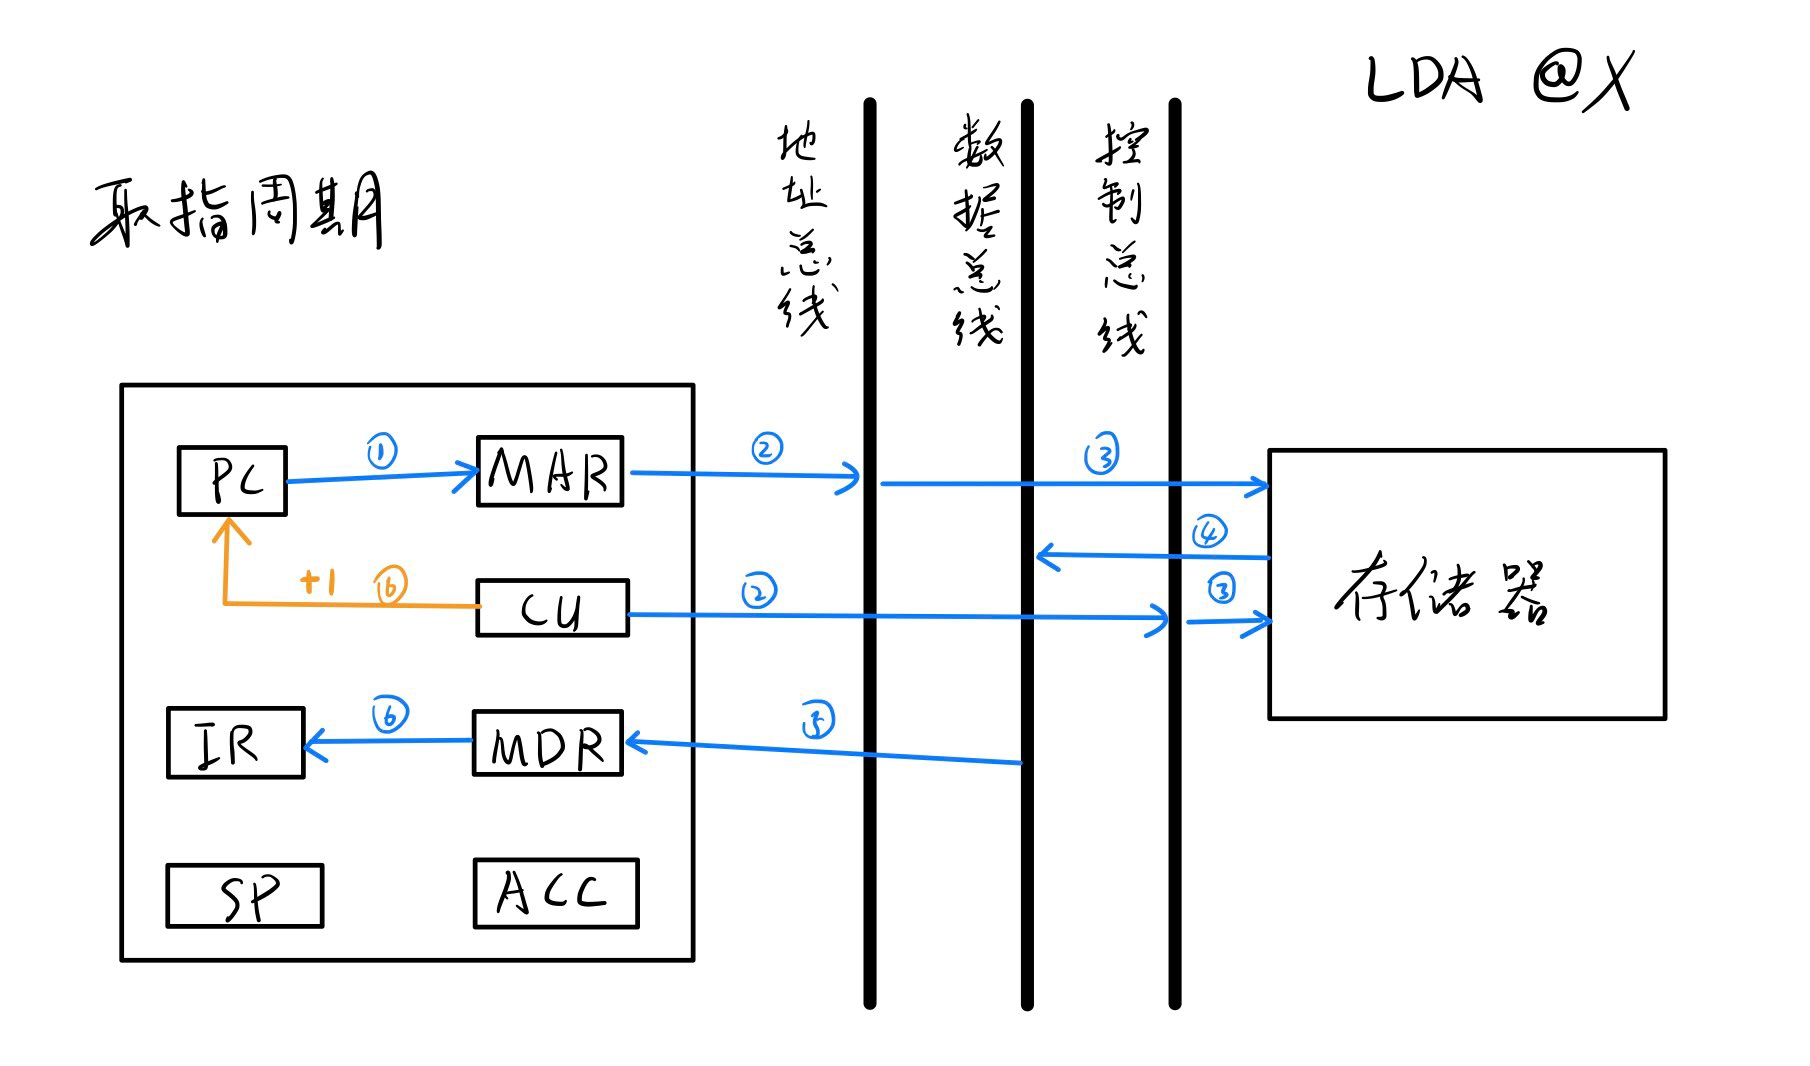
\includegraphics[width=9cm]{fig/8.4_1.png}
            \caption{题8.4 (1) 1}
            \label{fig:8_4_1}
        \end{figure}
        \newpage
        \begin{figure}[!htbp]
            \centering
            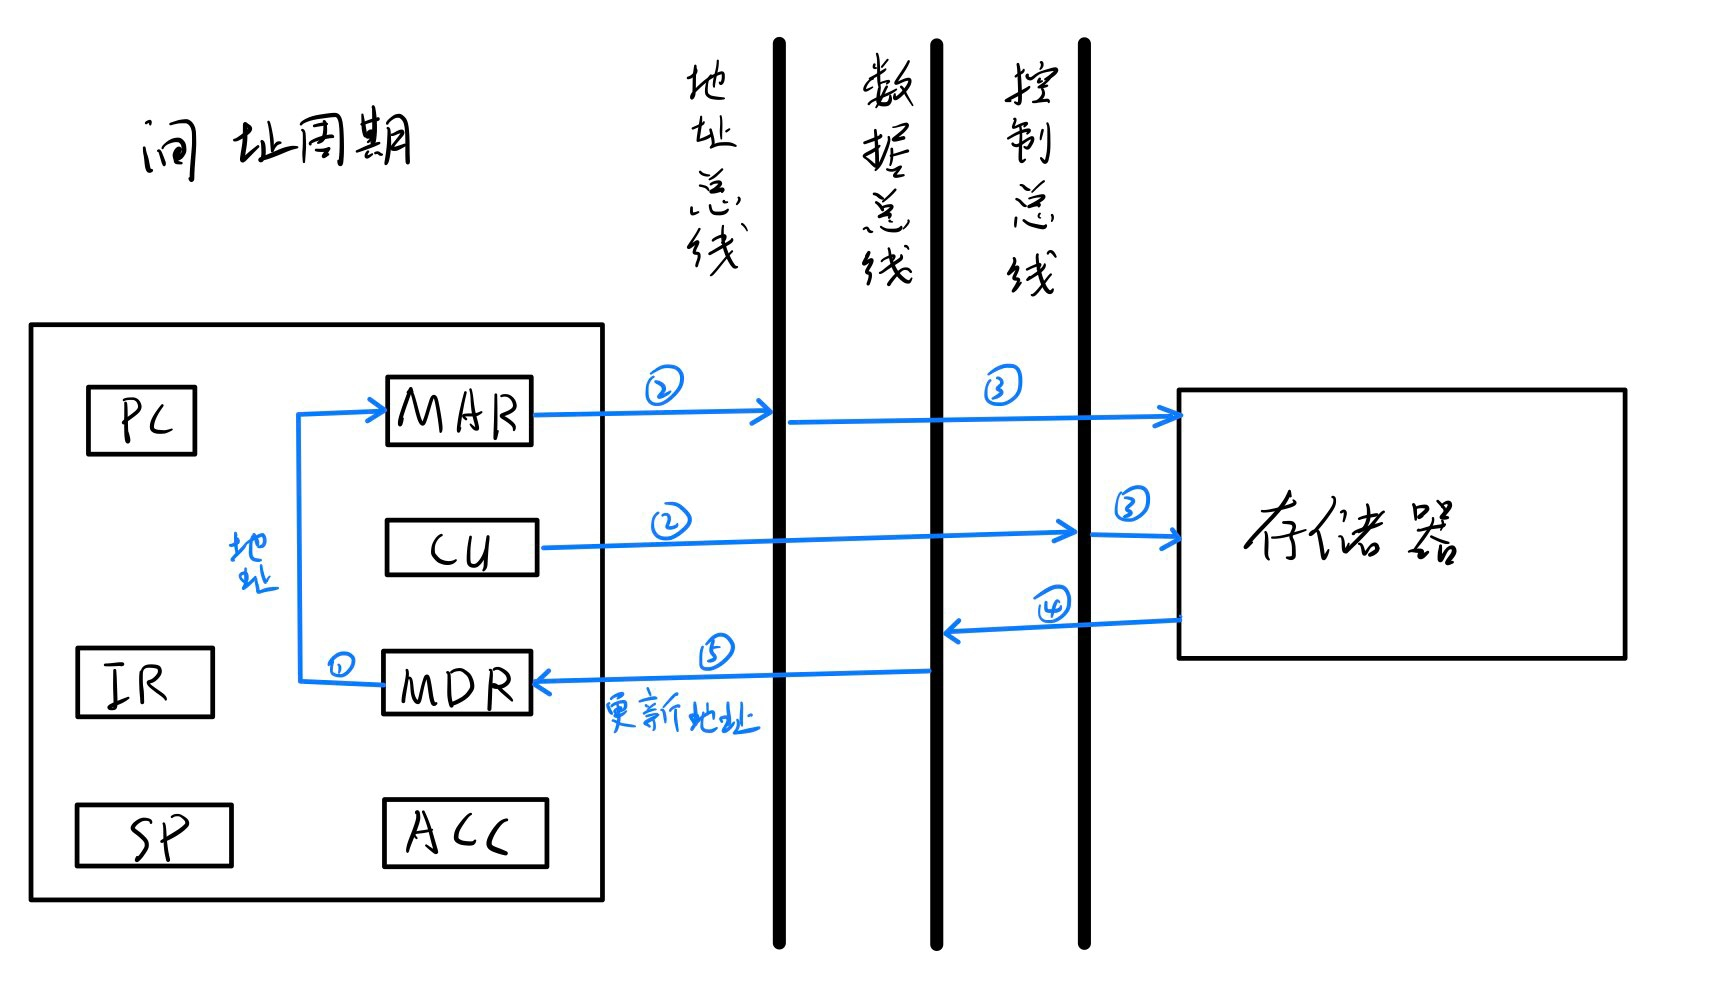
\includegraphics[width=9cm]{fig/8.4_2.png}
            \caption{题8.4 (1) 2}
            \label{fig:8_4_2}
        \end{figure}
        \begin{figure}[!htbp]
            \centering
            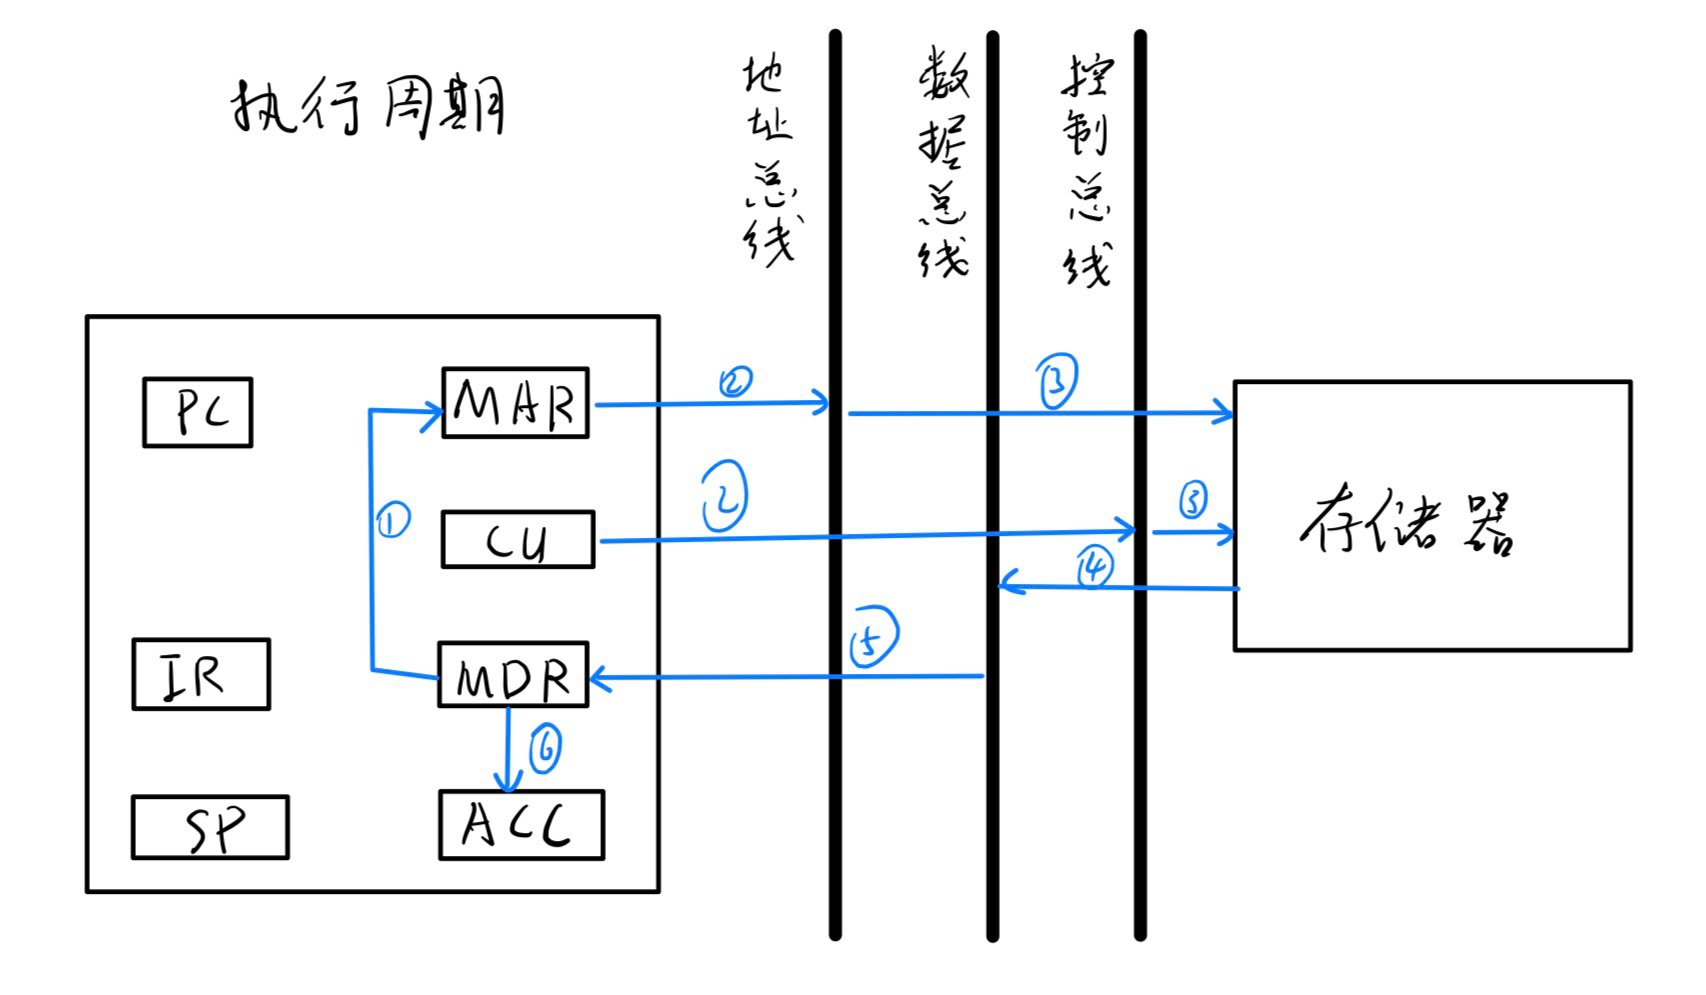
\includegraphics[width=9cm]{fig/8.4_3.png}
            \caption{题8.4 (1) 3}
            \label{fig:8_4_3}
        \end{figure}

        \item 如图

        \begin{figure}[!htbp]
            \centering
            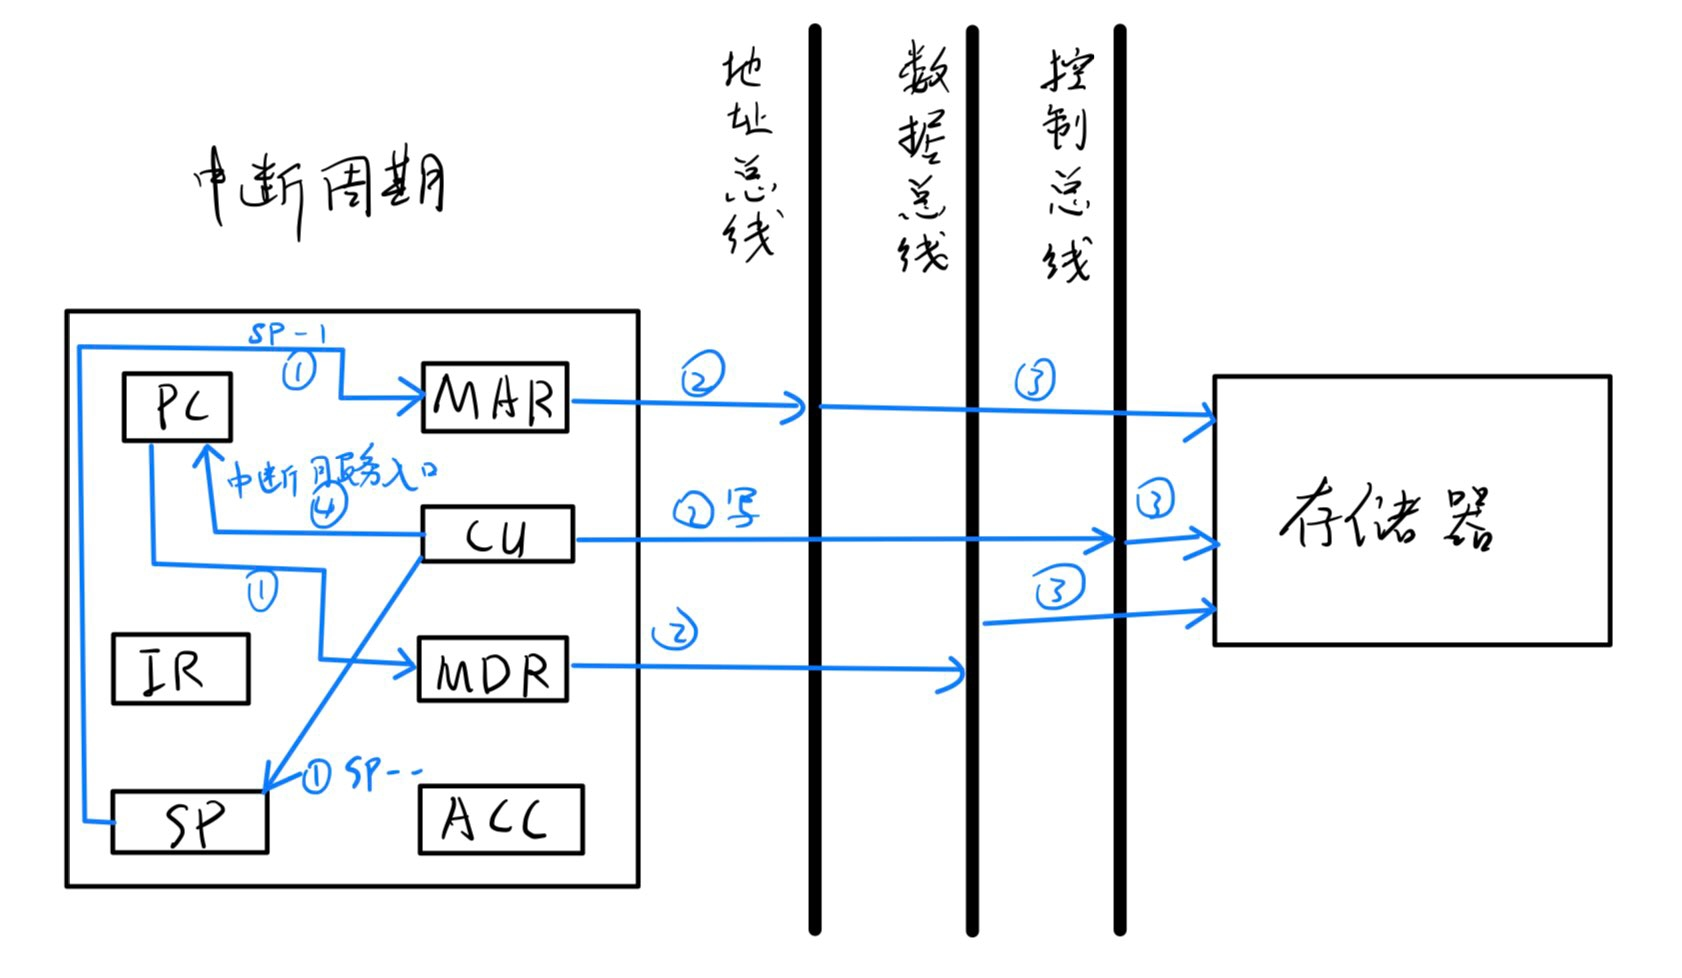
\includegraphics[width=9cm]{fig/8.4_4.png}
            \caption{题8.4 (2)}
            \label{fig:8_4_4}
        \end{figure}
    \end{enumerate}
\end{solution}

\newpage
    
\problem{8.8} 什么是指令流水?画出指令二级流水和四级流水的示意图,它们中哪一个更能提高处理器速度,为什么?

\begin{solution}
    % Table generated by Excel2LaTeX from sheet '草稿'
    \begin{table}[htbp]
        \centering
        \caption{指令的二级流水与四级流水对比}
        \begin{tabular}{lrrrrr|l|l|l|l|}
    \cline{2-3}    \multicolumn{1}{l|}{指令1} & \multicolumn{1}{l|}{取指} & \multicolumn{1}{l|}{执行} &   &   & \multicolumn{1}{r}{} & \multicolumn{1}{r}{} & \multicolumn{1}{r}{} & \multicolumn{1}{r}{} & \multicolumn{1}{r}{} \bigstrut\\
    \cline{2-4}    指令2 & \multicolumn{1}{r|}{} & \multicolumn{1}{l|}{取指} & \multicolumn{1}{l|}{执行} &   & \multicolumn{1}{r}{} & \multicolumn{1}{r}{} & \multicolumn{1}{r}{} & \multicolumn{1}{r}{} & \multicolumn{1}{r}{} \bigstrut\\
    \cline{3-5}    指令3 &   & \multicolumn{1}{r|}{} & \multicolumn{1}{l|}{取指} & \multicolumn{1}{l|}{执行} & \multicolumn{1}{r}{} & \multicolumn{1}{r}{} & \multicolumn{1}{r}{} & \multicolumn{1}{r}{} & \multicolumn{1}{r}{} \bigstrut\\
    \cline{4-6}    指令4 &   &   & \multicolumn{1}{r|}{} & \multicolumn{1}{l|}{取指} & \multicolumn{1}{l|}{执行} & \multicolumn{1}{r}{} & \multicolumn{1}{r}{} & \multicolumn{1}{r}{} & \multicolumn{1}{r}{} \bigstrut\\
    \cline{5-7}    指令5 &   &   &   & \multicolumn{1}{r|}{} & \multicolumn{1}{l|}{取指} & 执行 & \multicolumn{1}{r}{} & \multicolumn{1}{r}{} & \multicolumn{1}{r}{} \bigstrut\\
    \cline{6-8}    指令6 &   &   &   &   &   & 取指 & 执行 & \multicolumn{1}{r}{} & \multicolumn{1}{r}{} \bigstrut\\
    \cline{7-8}      &   &   &   &   & \multicolumn{1}{r}{} & \multicolumn{1}{r}{} & \multicolumn{1}{r}{} & \multicolumn{1}{r}{} & \multicolumn{1}{r}{} \bigstrut[t]\\
            &   &   &   &   & \multicolumn{1}{r}{} & \multicolumn{1}{r}{} & \multicolumn{1}{r}{} & \multicolumn{1}{r}{} & \multicolumn{1}{r}{} \bigstrut[b]\\
    \cline{2-5}    \multicolumn{1}{l|}{指令1} & \multicolumn{1}{l|}{取指} & \multicolumn{1}{l|}{译码取数} & \multicolumn{1}{l|}{执行} & \multicolumn{1}{l|}{写结果} & \multicolumn{1}{r}{} & \multicolumn{1}{r}{} & \multicolumn{1}{r}{} & \multicolumn{1}{r}{} & \multicolumn{1}{r}{} \bigstrut\\
    \cline{2-6}    指令2 & \multicolumn{1}{r|}{} & \multicolumn{1}{l|}{取指} & \multicolumn{1}{l|}{译码取数} & \multicolumn{1}{l|}{执行} & \multicolumn{1}{l|}{写结果} & \multicolumn{1}{r}{} & \multicolumn{1}{r}{} & \multicolumn{1}{r}{} & \multicolumn{1}{r}{} \bigstrut\\
    \cline{3-7}    指令3 &   & \multicolumn{1}{r|}{} & \multicolumn{1}{l|}{取指} & \multicolumn{1}{l|}{译码取数} & \multicolumn{1}{l|}{执行} & 写结果 & \multicolumn{1}{r}{} & \multicolumn{1}{r}{} & \multicolumn{1}{r}{} \bigstrut\\
    \cline{4-8}    指令4 &   &   & \multicolumn{1}{r|}{} & \multicolumn{1}{l|}{取指} & \multicolumn{1}{l|}{译码取数} & 执行 & 写结果 & \multicolumn{1}{r}{} & \multicolumn{1}{r}{} \bigstrut\\
    \cline{5-9}    指令5 &   &   &   & \multicolumn{1}{r|}{} & \multicolumn{1}{l|}{取指} & 译码取数 & 执行 & 写结果 & \multicolumn{1}{r}{} \bigstrut\\
    \cline{6-10}    指令6 &   &   &   &   &   & 取指 & 译码取数 & 执行 & 写结果 \bigstrut\\
    \cline{7-10}    \end{tabular}%
        \label{tab:addlabel}%
    \end{table}%

    四级流水更能提高效率. 因为它能将指令周期切分地更均匀, 能够使用更小的机器周期完成指令, 进而提高指令执行的速度.
\end{solution}


\problem{8.11} 今有四级流水线,分别完成取指(IF)、译码取数(ID)、执行(EX)、写结果(WR) 4个步骤。假设完成各步操作的时间依次为90ns、90ns、60ns、45ns。
\begin{enumerate}[label=(\arabic*)]
    \item 流水线的时钟周期应取何值?
    \item 若相邻的指令发生数据相关,那么第2 条指令安排推迟多少时间才能不发生错误?
    \item 若相邻两指令发生数据相关,为了不推迟第2 条指令的执行,可采取什么措施?
\end{enumerate}

\begin{solution}
    \begin{enumerate}[label=(\arabic*)]
        \item 90ns. 这是所有操作中最长的时间, 指令流水线必须要保证所有操作都能够完成.
        \item 180ns. 相邻两条指令的相关, 需要等待时间最长的情况, 可能是写后读情况, 第一条指令写的数据需要被第二条指令读取. 这种情况下, 第一条指令在执行时, 第二条指令就需要取数了. 我们应该推迟两个时钟周期, 让结果写完之后再拿来给数使用.
        \item 可以增加冲突处理模块. 比如写后读情况,  将第一条指令执行得到的结果直接送给第二条指令的取数, 省去推迟指令执行的麻烦.
    \end{enumerate}
\end{solution}


\problem{8.12}在5个功能段的指令流水线中,假设每段的执行时间分别是10ns、8ns、10ns、10ns和7ns。对于完成12条指令的流水线而言,其加速比为多少?该流水线的实际吞吐率为多少?

\begin{solution}
    流水线的时钟周期应该采用$10\unit{ns}$

    加速比: $n$条指令在$m$级流水线速度与等功能的非流水线速度之比. 

    \[
        S_p = \frac{(10+8+10+10+7)n}{10(n+m-1)} = \frac{(10+8+10+10+7) \times 12}{10 \times (12+5-1)} = \frac{27}{8} = 3.375
    \]

    实际吞吐率: $n$条指令在流水线中完成, 其实际的吞吐率 (单位时间内所能完成的指令数).

    \[
        T_p = \frac{n}{10(m+n-1)} = \frac{12}{10(5+12-1)} = \frac{3}{40} = 0.075 \unit{ns^{-1}}
    \]
\end{solution}




\end{document}